\section{Biconditional Statements}

\begin{itemize}
    \item Recall that "$P$ iff $Q$ is equivalent to "If $P$ then $Q$ and if $Q$ then $P$".
    \item If you want to write a biconditional proof, write a proof for if $P$ then $Q$ and then write another proof for if $Q$ then $P$. 
\end{itemize}

\begin{proposition}
    The integer $n$ is odd if and only if $n^2$ is odd. 
\end{proposition}

\begin{proof}
    \subsubsection*{$\implies$}


    \subsubsection{$\implies$}

    Suppose $n$ is even. This means there is some integer $k$ such that $n = 2k$. This means that $n^2 = (2k)^2 = 4k^2 = 2(2k^2)$. Since $k$ is an integer, then $2k^2$ is also an integer. 
\end{proof}


\section{Equivalence Statements}

\begin{itemize}
    \item This is a generalization of biconditional statements
    \item We will use the phrase "the following are equivalent" (TFAE)
\end{itemize}

\begin{theorem}[The Invertible Matrix Theorem]{theorem6.1.1:def}
    Let $A$ be a square matrix. Then the following statements are equivalent:

    \begin{enumerate}
        \item $A$ is invertible
        \item $A$ is row equivalent to the $n\times n$ identity matrix
        \item $A$ has $n$ pivot positions
        \item The equation $A\vec{x} = \vec{0}$ has only the trivial solution
        \item The columns of $A$ form a linearly indepentent set
        \item The linear transformation $\vec \rightarrow A\vec{x}$ is one-to-one
        \item The equation $A\vec{x} = \vec{b}$ has at least one solution for each $\vec{b}$ in $\R^n$
        \item The columns of $A$ span $\R^n$
        \item The linear transformation $\vec{x} \rightarrow A\vec{x}$ maps $\R^n$ onto $R^n$
        \item There is an $n\times n$ matrix $C$ such that $CA = I$
        \item There is an $n\times n$ matrix $D$ such that $AD = I$
        \item $A^T$ is invertible
    \end{enumerate}
\end{theorem}

    \begin{center}
        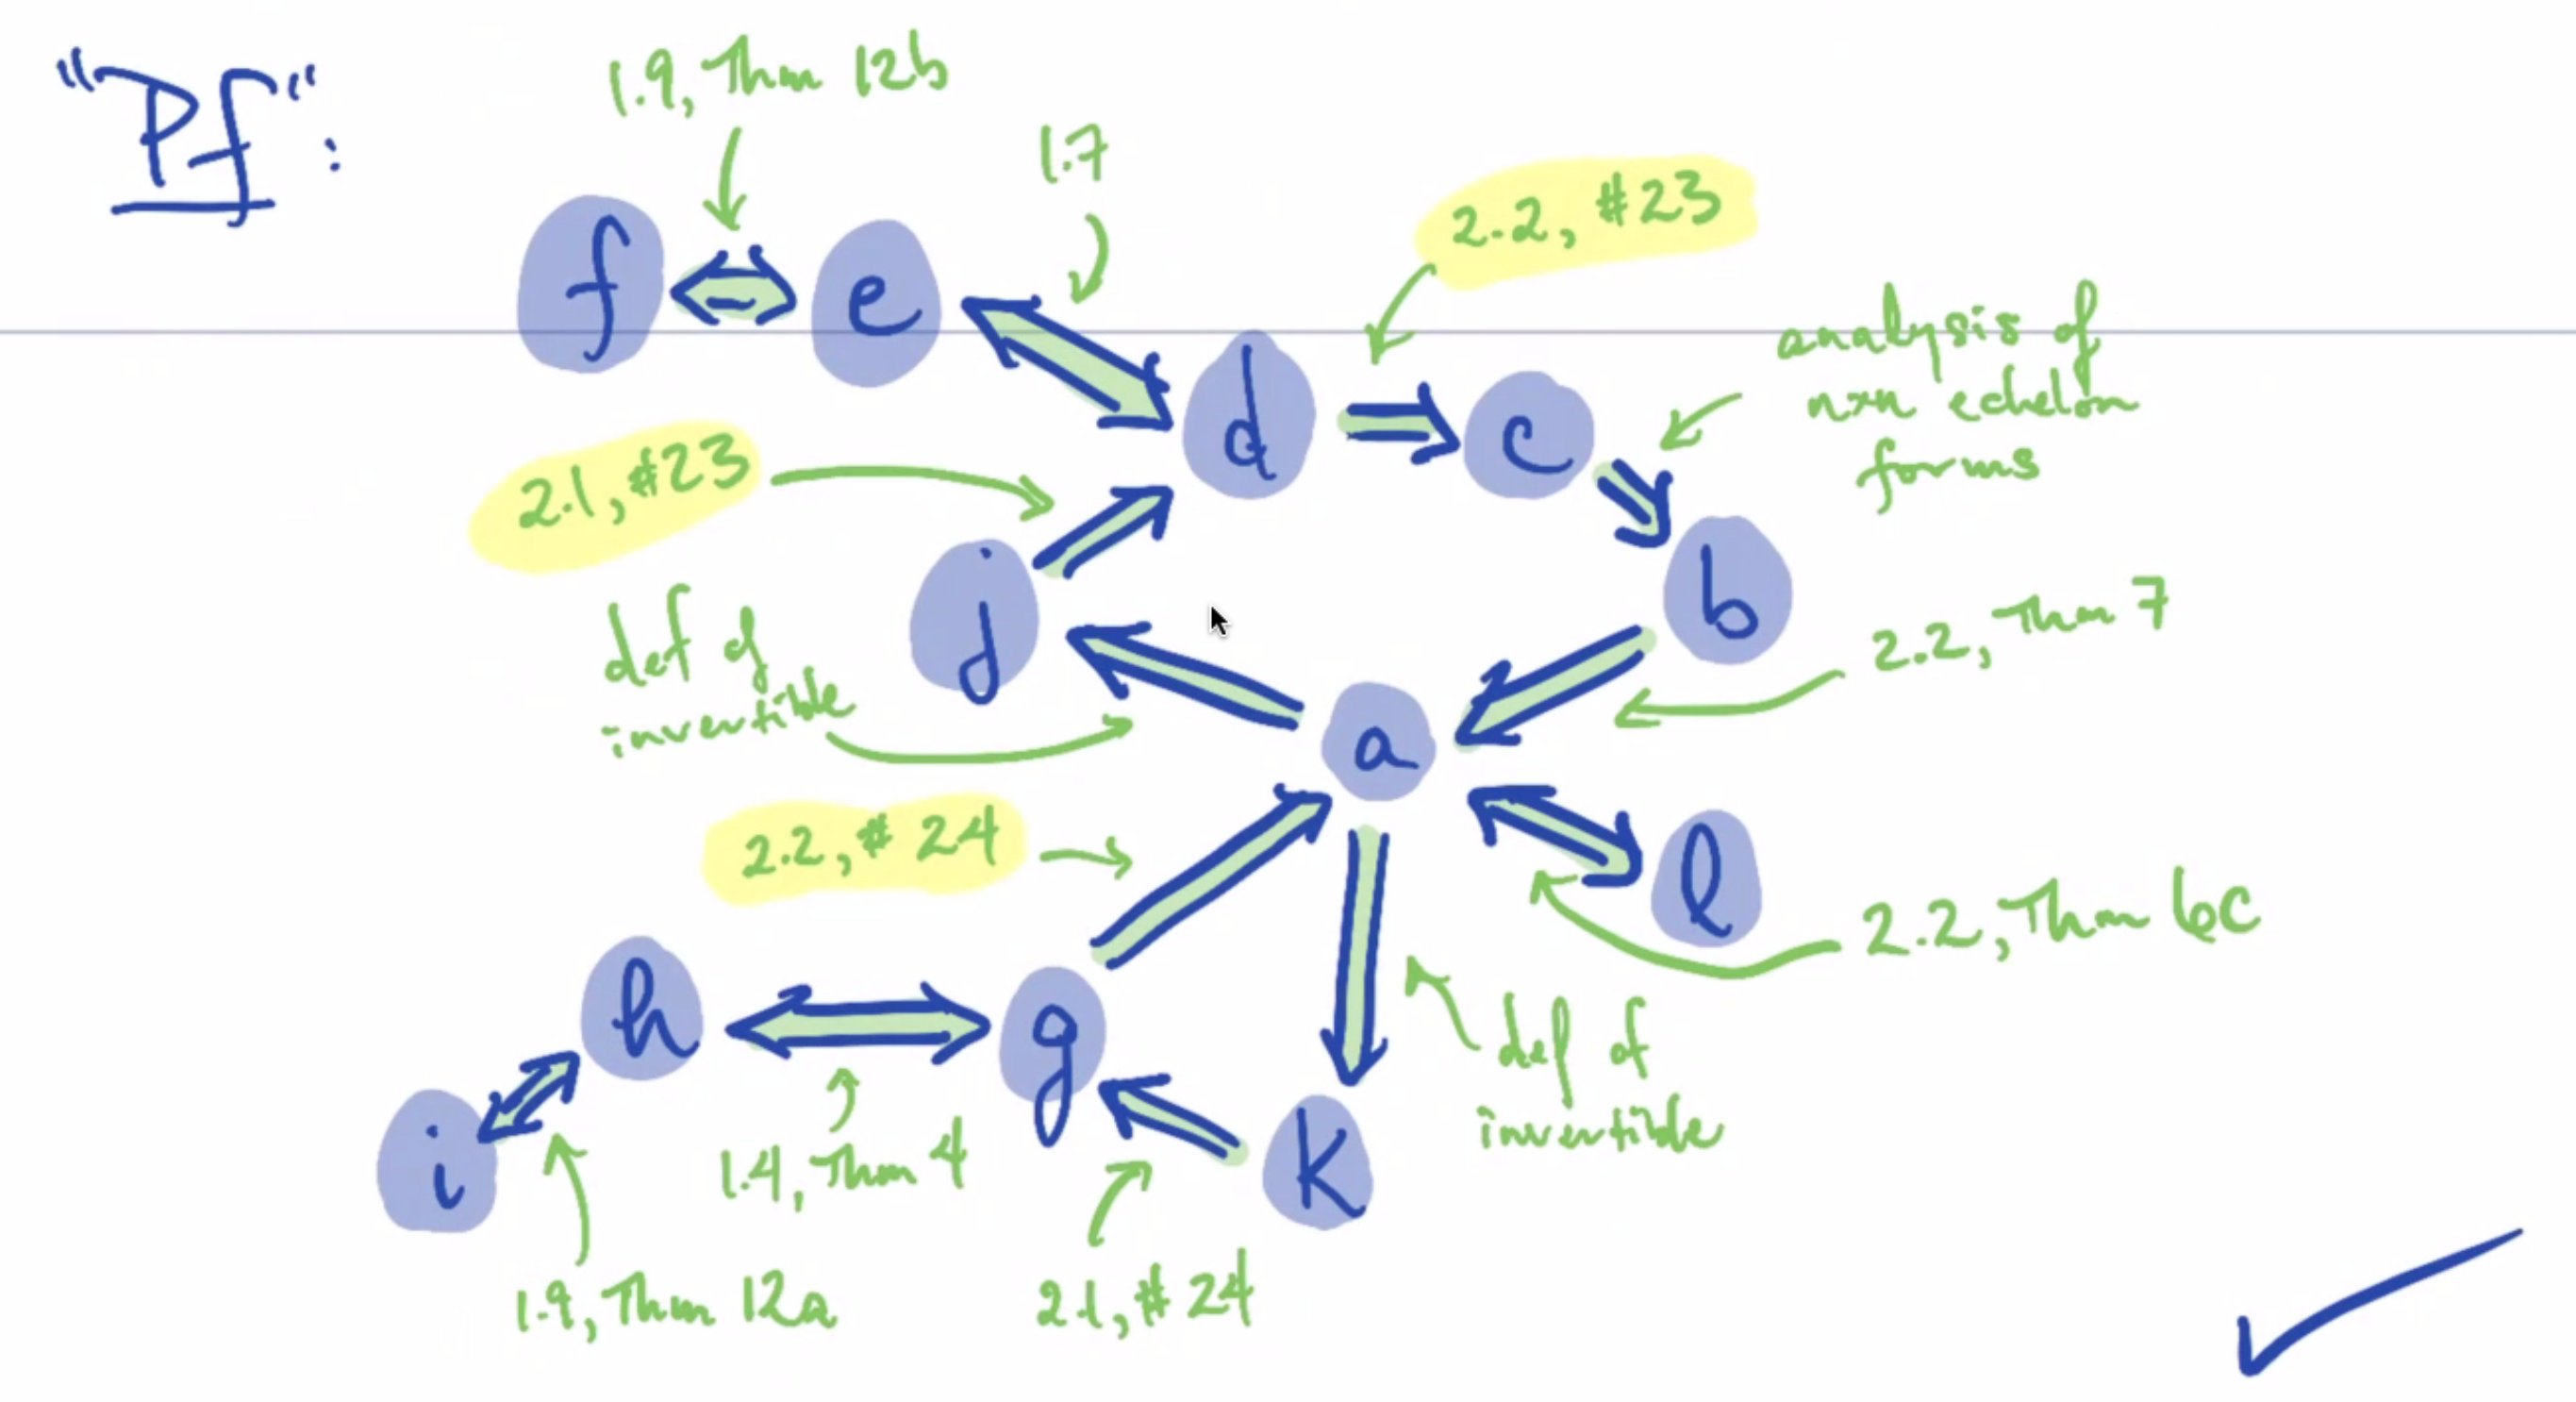
\includegraphics[width=1\textwidth]{chapters/ch6/images/fig6.1.PNG}
    \end{center}


\section{Existence and Uniqueness}

If you want to prove a statement such as $\exists x, P(x)$ or $\exists ! x, P(x)$, all you have to do is come up with one example that causes the statement to be true. This is the \textit{one} time that we are allowed to prove something by example!\\

There are two different types of proofs that fall under this category:

\begin{itemize}
    \item \textbf{constructive proofs:} Prove that the statement is true by constructing/showing one specific example. 
    \item \textbf{nonconstructive proofs:} show that the statement needs to exist, but you don't (or sometimes can't) give a specific example.
\end{itemize}


\begin{proposition}
    TThere is an even prime.
\end{proposition}

\begin{proof}
    (constructive proof) 2 is an even prime because $2=2\cdot 1$ is the only factorization of 2 which means it is prime, and it is even because it can be written as $2(1)$ which is two times some integer (the form of an even number). 
\end{proof}


\begin{proposition}
    FFor any set of five integers, there is a subset of three integers whose sum is a multiple of 3. 
\end{proposition}

\begin{proof}
    (nonconstructive proof) Let $S = \{a,b,c,d,e\}$, where $a,b,c,d,e\in\Z$. If any three elements of $S$ are equivalent mod 3, then we claim that their sum is divisible by 3. Suppose then that $a\equiv b\equiv c \mod 3$. Then for some $d \in \{0,1,2\}$ and for some $k,l,m\in\Z$, we have that $a=3k+d$, $b=3l+d$, $c=3m+d$. This means that:

    \[
        a+b+c = (3k+d) + (3l+d) + (3m+d) + 3(k+l+m) + 3d  
    \]

    Now, if there are not three equivalent numbers mod 3, it msut be that by the pigeonhole principle, there must be at least one number in each equivalence class mod 3. If, say, $a=3k$, $b=3l+1$, and $c=3m+2$ for some $k,lm\in\Z$, then:

    \[
        a + b + c = 3k + (3l+1) + (3m+2) = 3(k+l+m) + (1+2) = 3(k+l+m+1)  
    \]
\end{proof}